We will be implementing a prototype world builder over the course of one semester.
This prototype will stay true to the design, however, due to time constraints, not all features will be included.

\subsection{Physical Environment}
The physical environment remains the same between the end-goal and this prototype phase.
We will still be using a Head Mounted Display, along with two Wiimotes.
All will be independently tracked using a Vicon system in a 12ft x 22ft space.
Also, the Wiimotes provide 11 buttons each, that will be used for interaction and navigation (see Figure \ref{fig:wiimote}).

\subsection{Virtual Environment}
The virtual environment will still be an infinite world, with a goal of letting the user design any object, building, landscape, or geometrical feature they can imagine.
However, simulation effects such as gravity and animation will not be included.
The user can still create objects and place them together to make more complex and larger objects, but they will not be able to give them motion.

Sound and light creation/manipulation were not implemented in the prototype though a fully featured World Builder IVE would have these capabilities.

\subsection{Interaction}
During this prototype phase, the most important aspect is the interaction abilities the user has.

\subsubsection{Selection}
We implemented our own hybrid technique which we call Virtual Hand Casting.
The ray from each hand is drawn to infinity then for each object we calculate the closest point on the ray to the center of that object.
We then determine if the point on the line is within the bounding sphere of the object.
The object who's point on the ray is closest to the user's hand is determined to be the object being pointed at by the user.
This selection technique works extremely well provided that an object isn't fully within the bounding sphere of another object.
Since PORT is not being provided in the prototype, multi object selection will require the user to select objects in turn.

\subsubsection{Manipulation}
\paragraph{Single-Object Manipulation}
All features discussed in the design section for single object manipulation will be included.
The user will be able to create, delete, translate, rotate, scale and texture all objects within the world.

\paragraph{Multi-Object Manipulation}
Boolean operations will not be provided in the prototype.
However, the user will be able to group multiple objects to form a single object, and delete multiple selected objects.

\paragraph{World Manipulation}
Scale-the-World will be provided.
This feature is essential given that the size of the world is so big, and the user will need to navigate large spaces.

\subsubsection{Navigation}
Both real walking and virtual walking will be provided.
Real walking is accomplished by the framework with little effort.
Virtual walking will use the D-Pad and move the origin point of the environment, thereby moving the user through it.

Since Scale-the-World is provided, as well as both walking schemes, the user will be able to magnify their steps using the method described in \ref{Design:Interaction:Navigation}.

\subsubsection{System Control}
Many of the features described in \ref{Design:Interaction} require a menu, so a menu will be provided.
However, this will be simpler than the menu described in \ref{Design:Interaction}.
An object category and material category will be provided, as well as a tools category.
The tools category will only contain the features described in this section, namely, deletion and grouping.

If time permits, the file category will be provided that will allow the user to save/load the world they have spent time to create.

\subsection{Implementation}
We will be implementing the World Builder application using the \href{http://syzygy.isl.uiuc.edu/szg/szgsrc/doc/index.html}{Syzygy} virtual reality API created at the University of Illinois for the development.
This API allows us to do rapid prototype development, since some of the most complex features of an immersive virtual environment have been completed, including head based rendering, interaction with objects, and input device drivers.

The Syzygy API contains two frameworks that are used for development, \verb|arMasterSlaveFramework| and \verb|arDistSceneGraphFramework|.
We will be using the \verb|arMasterSlaveFramework|, but we are using a helper class created by the FIVE lab at UTD to include a Scene Graph in an \verb|arMasterSlaveFramework|.

\subsection{Extra Features}
This is a list of extra features we added to our prototype after usability testing. We determined that these would help usability or enhance the merriment aspect amongst the users.

\begin{itemize}
    \item laser pointer
    \item copy/paste of objects
    \item multiple object selection
    \item double speed
    \item bounding sphere object(s) being pointed at or selected
    \item grid on ``ground''
    \item center pole to illustrate both the start point as well as help the user visualize the current scale
\end{itemize}

\begin{figure}[htbp]
	\centering
	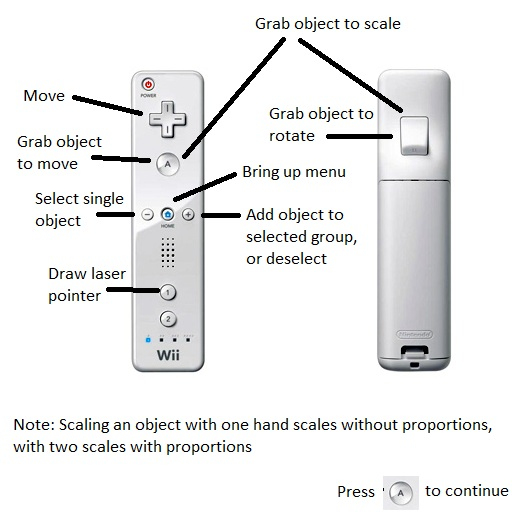
\includegraphics[width=3in]{figs/help.jpg}
	\caption{Input}
	\label{fig:help}
\end{figure}
